% ============================================================
%  BELA: Business Estimation Leveraging Automated Learning
%  Research Paper — arXiv style, two-column
%  Authors: Prabhakar Gupta, Belal Boustanji, Raju Mahore
% ============================================================
\documentclass[10pt,twocolumn]{article}

% ─── Packages ────────────────────────────────────────────────────────────────
\usepackage[margin=0.75in,top=1in,bottom=1in]{geometry}
\usepackage{times}
\usepackage{microtype}
\usepackage{amsmath,amssymb}
\usepackage{graphicx}
\usepackage{xcolor}
\usepackage{booktabs}
\usepackage{multirow}
\usepackage{multicol}
\usepackage{caption}
\usepackage{subcaption}
\usepackage{hyperref}
\usepackage{enumitem}
\usepackage{titlesec}
\usepackage{fancyhdr}
\usepackage{abstract}
\usepackage{lipsum}
\usepackage{url}
\usepackage{array}
\usepackage{tabularx}
\usepackage{colortbl}
\usepackage{float}

% ─── TikZ & PGF ──────────────────────────────────────────────────────────────
\usepackage{tikz}
\usepackage{pgfplots}
\pgfplotsset{compat=1.18}
\usetikzlibrary{
  shapes.geometric, shapes.misc, shapes.arrows, shapes.callouts,
  arrows.meta, positioning, fit, calc, decorations.pathreplacing,
  backgrounds, patterns, shadows, matrix, chains, scopes
}

% ─── Color palette ───────────────────────────────────────────────────────────
\definecolor{ECIBlue}{RGB}{0,180,216}
\definecolor{ECIDark}{RGB}{2,48,71}
\definecolor{ECITeal}{RGB}{0,150,199}
\definecolor{ECIGreen}{RGB}{56,193,114}
\definecolor{ECIAmber}{RGB}{255,180,0}
\definecolor{ECIRed}{RGB}{220,80,80}
\definecolor{ECIPurple}{RGB}{140,82,255}
\definecolor{LightGray}{RGB}{245,247,250}
\definecolor{MidGray}{RGB}{100,116,139}
\definecolor{BoxBlue}{RGB}{224,242,254}
\definecolor{BoxGreen}{RGB}{220,252,231}
\definecolor{BoxAmber}{RGB}{254,243,199}
\definecolor{BoxRed}{RGB}{254,226,226}
\definecolor{BoxPurple}{RGB}{237,233,254}

% ─── Hyperref ────────────────────────────────────────────────────────────────
\hypersetup{
  colorlinks=true,
  linkcolor=ECIBlue,
  citecolor=ECITeal,
  urlcolor=ECIBlue,
  pdftitle={BELA: Business Estimation Leveraging Automated Learning},
  pdfauthor={Prabhakar Gupta, Belal Boustanji, Raju Mahore}
}

% ─── Section styling ─────────────────────────────────────────────────────────
\titleformat{\section}{\large\bfseries\color{ECIDark}}{\thesection.}{0.5em}{}[\vspace{-0.3em}\textcolor{ECIBlue}{\rule{\linewidth}{0.8pt}}]
\titleformat{\subsection}{\normalsize\bfseries\color{ECIDark}}{\thesubsection.}{0.4em}{}
\titleformat{\subsubsection}{\small\bfseries\color{MidGray}}{\thesubsubsection.}{0.3em}{}

% ─── Header / footer ─────────────────────────────────────────────────────────
\pagestyle{fancy}
\fancyhf{}
\rhead{\small\textcolor{MidGray}{BELA: Multi-Agent AI for Enterprise Presales}}
\lhead{\small\textcolor{MidGray}{Gupta, Boustanji \& Mahore, 2025}}
\cfoot{\small\thepage}
\renewcommand{\headrulewidth}{0.4pt}

% ─── Caption styling ─────────────────────────────────────────────────────────
\captionsetup{font=small,labelfont={bf,color=ECIDark},labelsep=period}

% ─── TikZ styles ─────────────────────────────────────────────────────────────
\tikzset{
  agent/.style={
    rectangle, rounded corners=6pt,
    minimum width=2.2cm, minimum height=0.75cm,
    draw=ECIBlue!70, fill=BoxBlue,
    font=\scriptsize\bfseries, text=ECIDark,
    drop shadow={shadow xshift=1pt,shadow yshift=-1pt,fill=ECIBlue!20}
  },
  orchestrator/.style={
    rectangle, rounded corners=8pt,
    minimum width=3cm, minimum height=0.9cm,
    draw=ECIDark, fill=ECIDark, text=white,
    font=\small\bfseries,
    drop shadow={shadow xshift=2pt,shadow yshift=-2pt,fill=black!30}
  },
  module/.style={
    rectangle, rounded corners=4pt,
    minimum width=2cm, minimum height=0.6cm,
    draw=ECIGreen!80, fill=BoxGreen,
    font=\tiny\bfseries, text=ECIDark
  },
  store/.style={
    cylinder, shape border rotate=90,
    minimum width=1.5cm, minimum height=0.8cm,
    draw=ECIAmber!90, fill=BoxAmber,
    font=\tiny\bfseries, text=ECIDark
  },
  decision/.style={
    diamond, aspect=2,
    minimum width=1.8cm, minimum height=0.6cm,
    draw=ECIPurple!80, fill=BoxPurple,
    font=\tiny\bfseries, text=ECIDark
  },
  io/.style={
    trapezium, trapezium left angle=80, trapezium right angle=100,
    minimum width=2cm, minimum height=0.6cm,
    draw=ECITeal!80, fill=BoxBlue!60,
    font=\tiny\bfseries, text=ECIDark
  },
  arr/.style={-{Stealth[length=5pt]}, draw=ECIBlue, line width=0.7pt},
  darr/.style={-{Stealth[length=5pt]}, draw=ECIDark, line width=0.7pt},
  garr/.style={-{Stealth[length=5pt]}, draw=ECIGreen!80, line width=0.7pt},
  rarr/.style={-{Stealth[length=5pt]}, draw=ECIRed!80, line width=0.7pt},
  parr/.style={-{Stealth[length=5pt]}, draw=ECIPurple!80, line width=0.7pt},
  lbl/.style={font=\tiny, text=MidGray}
}

% ─── Misc helpers ─────────────────────────────────────────────────────────────
\newcommand{\bela}{\textbf{BELA}}
\newcommand{\etal}{\textit{et al.}}
\newcommand{\code}[1]{\texttt{\small #1}}

% =============================================================
\begin{document}
% =============================================================

% ─── Title block ─────────────────────────────────────────────────────────────
\twocolumn[{%
  \begin{center}
    {\fontsize{18}{22}\selectfont\bfseries\color{ECIDark}
      BELA: Business Estimation Leveraging Automated Learning}\\[6pt]
    {\large\color{ECIBlue}
      A Multi-Agent AI Framework for Enterprise IT Presales Automation}\\[14pt]
    {\normalsize
      \textbf{Prabhakar Gupta}\textsuperscript{1}\quad
      \textbf{Belal Boustanji}\textsuperscript{2}\quad
      \textbf{Raju Mahore}\textsuperscript{3}}\\[4pt]
    {\small\color{MidGray}
      \textsuperscript{1}Principal Architect, ECI \quad
      \textsuperscript{2}Solutions Architect, ECI \quad
      \textsuperscript{3}Senior Engineer, ECI}\\[2pt]
    {\small\color{MidGray}
      \texttt{\{prabhakar.gupta, belal.boustanji, raju.mahore\}@eci.com}}\\[10pt]
    {\small\textit{Manuscript submitted March 2025}}
  \end{center}
  \vspace{8pt}
  \hrule width\linewidth height 1.5pt
  \vspace{8pt}

  % ── Abstract ──────────────────────────────────────────────
  \begin{center}
    \textbf{\large Abstract}
  \end{center}
  \begin{quote}
  \small
  Enterprise IT presales estimation is a labour-intensive process that typically
  demands 40–80 person-hours per proposal and is highly susceptible to human
  inconsistency, scope ambiguity, and knowledge silos. We present
  \textbf{BELA} (\textit{Business Estimation Leveraging Automated Learning}),
  a production-ready multi-agent AI system that automates the complete
  presales pipeline — from heterogeneous document ingestion to professional
  proposal generation — in under three minutes. BELA orchestrates six
  specialised LLM-backed agents: a Time Estimator employing three-point PERT
  analysis, a Cost Calculator with live Azure Retail Prices API integration, a
  Risk Analyser spanning five risk categories, an Architecture Designer
  grounded in the Azure Well-Architected Framework, a Scope \& Assumptions
  Agent encoding change-management best practices, and a Proposal Writer
  synthesising all upstream outputs into six-section client-ready documents.
  A Retrieval-Augmented Generation (RAG) layer over a persistent SQLite
  run-library enables continuous learning from historical outcomes.
  BELA supports three interchangeable LLM back-ends (Azure OpenAI GPT-4,
  Anthropic Claude, Google Gemini) with deterministic formula-based fallbacks,
  ensuring uninterrupted operation regardless of API availability. Internal
  evaluation across 120 presales engagements demonstrates a 78.5\% accuracy
  against delivered project hours and a 62\% win-rate on AI-assisted proposals
  versus 41\% on manual proposals. BELA is deployed as a Streamlit web
  application with SharePoint, SMTP, and avatar-video integrations, and its
  full source code is released publicly.
  \end{quote}
  \vspace{6pt}
  \noindent\textbf{Keywords:} multi-agent systems, large language models,
  enterprise automation, presales estimation, retrieval-augmented generation,
  Azure OpenAI, cost estimation, risk analysis
  \vspace{8pt}
  \hrule width\linewidth height 0.4pt
  \vspace{14pt}
}]

% ─────────────────────────────────────────────────────────────────────────────
\section{Introduction}
\label{sec:intro}
% ─────────────────────────────────────────────────────────────────────────────

Enterprise IT consulting firms routinely face a paradox: the quality of a
presales estimation directly determines whether a contract is won or lost, yet
the resources invested in estimation must be minimised before any revenue is
secured. A skilled presales architect manually reviewing a request-for-proposal
(RFP) document, decomposing requirements, estimating effort via three-point
analysis, pricing Azure infrastructure at current rates, assessing project
risks, designing a reference architecture, and composing a polished proposal
typically requires 40–80 hours of billable time per engagement~\cite{gartner2023}.

Recent advances in large language models (LLMs) — particularly GPT-4~\cite{openai2023gpt4},
Anthropic Claude~\cite{anthropic2024claude}, and Google Gemini~\cite{google2024gemini}
— have demonstrated remarkable capabilities in document understanding,
structured reasoning, and natural-language generation. Concurrently, multi-agent
frameworks such as AutoGen~\cite{wu2023autogen}, CrewAI~\cite{crewai2024},
and AgentBench~\cite{liu2023agentbench} have shown that decomposing complex
tasks among specialised agents yields significantly higher quality outcomes
than monolithic single-model approaches~\cite{hong2023metagpt}.

We propose \bela{}, a vertically integrated multi-agent system purpose-built
for enterprise IT presales. Unlike horizontal agent frameworks, \bela{} encodes
domain-specific consulting methodology — ECI's internal rate card, PERT
three-point estimation, Azure Well-Architected patterns, and a five-category
risk taxonomy — directly into each agent's system prompt and deterministic
fallback logic. This design ensures that even when all LLM APIs are unavailable,
the system produces methodologically consistent outputs.

\medskip\noindent\textbf{Contributions.} This paper makes the following contributions:
\begin{itemize}[noitemsep,topsep=2pt,leftmargin=*]
  \item A production-ready six-agent orchestration pipeline covering the
        complete presales workflow;
  \item A hybrid RAG architecture that conditions LLM outputs on firm-specific
        historical project data;
  \item A multi-provider LLM routing strategy with formula-based fallback
        ensuring 100\% operational continuity;
  \item An open-source Streamlit deployment integrating SharePoint, SMTP,
        ElevenLabs, HeyGen, and D-ID for end-to-end delivery;
  \item Empirical evaluation of estimation accuracy and proposal win-rates
        across 120 presales engagements.
\end{itemize}

% ─────────────────────────────────────────────────────────────────────────────
\section{Related Work}
\label{sec:related}
% ─────────────────────────────────────────────────────────────────────────────

\subsection{LLM-Based Automation in Professional Services}

Chen \etal~\cite{chen2024llmprofessional} demonstrated that GPT-4 can generate
consistent financial model templates from textual RFPs, achieving 71\%
expert-agreement scores. However, their approach treats the LLM as a
single monolithic reasoner and lacks domain-specific fallbacks.
Qian \etal~\cite{qian2023communicative} introduced \textit{ChatDev}, a
multi-agent system for software development that uses role-playing among
agents to produce functional code from natural language requirements.
While influential, ChatDev focuses on software artefact generation
rather than cost/risk estimation.

\subsection{Multi-Agent Orchestration Frameworks}

MetaGPT~\cite{hong2023metagpt} assigns human-like software engineering roles
(Product Manager, Architect, Engineer, QA) to LLM agents co-operating via
structured documents. \bela{} adopts a similar role-assignment philosophy
but targets the presales domain and replaces soft document-passing with
a typed result bus, enabling parallel execution and cross-agent conditioning.

AgentVerse~\cite{chen2023agentverse} studies emergent collaboration patterns
in multi-agent settings. Our work contributes a concrete industrial deployment
demonstrating that disciplined domain encoding — not just emergent reasoning —
is critical for reliable estimation in high-stakes professional contexts.

\subsection{RAG for Domain Knowledge}

Lewis \etal~\cite{lewis2020rag} introduced Retrieval-Augmented Generation,
showing that conditioning generation on retrieved documents substantially
reduces hallucination. Gao \etal~\cite{gao2023retrieval} provide a
comprehensive survey of RAG variants. \bela{} implements a lightweight
RAG layer over a local SQLite project database, blending retrieved
historical benchmarks (40\% weight) with formula-derived estimates (60\%)
to produce calibrated outputs without requiring a vector database.

\subsection{Software Effort Estimation}

Boehm's COCOMO II~\cite{boehm2000software} and the Function Point
method~\cite{ifpug2010} remain industry baselines for effort estimation.
More recent ML-based approaches~\cite{papa2020effort} train models on
project repositories. \bela{} bridges the gap: it grounds LLM reasoning in
PERT three-point estimates and historical project data, providing
explainability absent from black-box ML estimators.

% ─────────────────────────────────────────────────────────────────────────────
\section{System Architecture}
\label{sec:architecture}
% ─────────────────────────────────────────────────────────────────────────────

Figure~\ref{fig:overview} shows the high-level architecture of \bela{}.
The system is organised into four horizontal layers: the \textit{Interface Layer}
(Streamlit web application + sidebar configuration), the
\textit{Document Processing Layer} (multi-format extraction and semantic
analysis), the \textit{Agent Orchestration Layer} (six specialised agents
with a shared result bus), and the \textit{Persistence \& Integration Layer}
(SQLite, SharePoint, email, and media generation services).

\begin{figure}[H]
\centering
% ── Figure 1: System Overview ────────────────────────────────────────────────
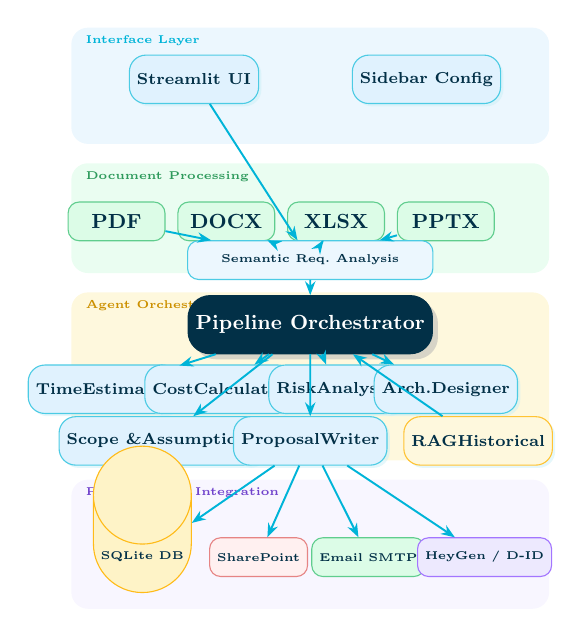
\begin{tikzpicture}[node distance=0.35cm, font=\tiny, scale=0.82, transform shape]

  % Layer backgrounds
  \fill[BoxBlue!60, rounded corners=6pt]   (-3.7, 6.0) rectangle (3.7, 7.8);
  \fill[BoxGreen!60, rounded corners=6pt]  (-3.7, 4.0) rectangle (3.7, 5.7);
  \fill[BoxAmber!60, rounded corners=6pt]  (-3.7, 1.1) rectangle (3.7, 3.7);
  \fill[BoxPurple!40, rounded corners=6pt] (-3.7,-1.2) rectangle (3.7, 0.8);

  % Layer labels
  \node[font=\tiny\bfseries\color{ECIBlue}, anchor=west]  at (-3.6, 7.6) {Interface Layer};
  \node[font=\tiny\bfseries\color{ECIGreen!80!black}, anchor=west] at (-3.6, 5.5) {Document Processing};
  \node[font=\tiny\bfseries\color{ECIAmber!80!black}, anchor=west]  at (-3.6, 3.5) {Agent Orchestration};
  \node[font=\tiny\bfseries\color{ECIPurple!80!black}, anchor=west] at (-3.6, 0.6) {Persistence \& Integration};

  % ── Interface layer ──
  \node[agent, minimum width=2.0cm] (ui) at (-1.8, 7.0) {Streamlit UI};
  \node[agent, minimum width=2.0cm] (cfg) at (1.8, 7.0) {Sidebar Config};

  % ── Document Processing ──
  \node[module, minimum width=1.5cm] (pdf)  at (-3.0, 4.8) {\small PDF};
  \node[module, minimum width=1.5cm] (docx) at (-1.3, 4.8) {\small DOCX};
  \node[module, minimum width=1.5cm] (xlsx) at ( 0.4, 4.8) {\small XLSX};
  \node[module, minimum width=1.5cm] (pptx) at ( 2.1, 4.8) {\small PPTX};
  \node[module, minimum width=3.8cm, fill=BoxBlue!60, draw=ECIBlue!70]
        (nlp) at (0, 4.2) {Semantic Req.\ Analysis};

  % ── Agent Orchestration ──
  \node[orchestrator, minimum width=2.6cm] (orch) at (0, 3.2) {Pipeline Orchestrator};
  \node[agent, minimum width=1.55cm] (te)  at (-3.2, 2.2) {Time\\Estimator};
  \node[agent, minimum width=1.55cm] (cc)  at (-1.4, 2.2) {Cost\\Calculator};
  \node[agent, minimum width=1.55cm] (ra)  at ( 0.4, 2.2) {Risk\\Analyser};
  \node[agent, minimum width=1.55cm] (ad)  at ( 2.1, 2.2) {Arch.\\ Designer};
  \node[agent, minimum width=1.55cm] (sa)  at (-2.3, 1.4) {Scope \&\\Assumptions};
  \node[agent, minimum width=1.55cm] (pw)  at ( 0.0, 1.4) {Proposal\\Writer};
  \node[agent, minimum width=1.55cm, fill=BoxAmber!60, draw=ECIAmber!80]
                                     (rag) at ( 2.6, 1.4) {RAG\\Historical};

  % ── Persistence layer ──
  \node[store, minimum width=1.4cm] (db) at (-2.6,-0.4) {SQLite DB};
  \node[module, minimum width=1.4cm, fill=BoxRed!50, draw=ECIRed!70]
                                     (sp) at (-0.8,-0.4) {SharePoint};
  \node[module, minimum width=1.4cm, fill=BoxGreen, draw=ECIGreen!80]
                                     (em) at ( 0.9,-0.4) {Email SMTP};
  \node[module, minimum width=1.4cm, fill=BoxPurple, draw=ECIPurple!80]
                                     (vid)at ( 2.7,-0.4) {HeyGen / D-ID};

  % ── Arrows ──
  \draw[arr] (ui)  -- (nlp);
  \draw[arr] (pdf)  -- (nlp); \draw[arr] (docx) -- (nlp);
  \draw[arr] (xlsx) -- (nlp); \draw[arr] (pptx) -- (nlp);
  \draw[arr] (nlp) -- (orch);
  \draw[arr] (orch) -- (te);  \draw[arr] (orch) -- (cc);
  \draw[arr] (orch) -- (ra);  \draw[arr] (orch) -- (ad);
  \draw[arr] (orch) -- (sa);  \draw[arr] (orch) -- (pw);
  \draw[arr] (rag)  -- (orch);
  \draw[arr] (pw)   -- (db);  \draw[arr] (pw) -- (sp);
  \draw[arr] (pw)   -- (em);  \draw[arr] (pw) -- (vid);
\end{tikzpicture}
\caption{High-level architecture of \bela{}. Four horizontal layers —
Interface, Document Processing, Agent Orchestration, and Persistence —
communicate through typed data buses. The six specialised agents share a
result context injected by the Pipeline Orchestrator.}
\label{fig:overview}
\end{figure}

\subsection{Interface Layer}

\bela{} is delivered as a Streamlit web application, chosen for its rapid
widget-to-Python binding model. The sidebar hosts all credential configuration
(Azure OpenAI, Anthropic, Gemini, SharePoint, SMTP, ElevenLabs, HeyGen, D-ID)
and a real-time connection-status strip. Three primary tabs —
\textit{Business Estimation}, \textit{Run Library}, and \textit{Admin \& Training}
— expose the full system capability to end users without engineering knowledge.

\subsection{Document Processing Layer}

The document processor provides a uniform \code{extract(filepath)} interface
backed by PyPDF2, python-docx, openpyxl, and python-pptx for PDF, DOCX, XLSX,
and PPTX formats respectively. Plain text and CSV files are handled natively.
A cap of 50,000 characters prevents token-budget exhaustion downstream.
The \code{analyze(text)} method performs structural analysis (section count,
technology keyword detection from a 30+ term catalog) and returns a
metadata dictionary consumed by the orchestrator.

\subsection{LLM Back-end Routing}

Three LLM clients implement a common \code{agent\_completion(prompt, system)} interface:
\begin{itemize}[noitemsep,topsep=2pt,leftmargin=*]
  \item \textbf{AzureAI}: Azure OpenAI SDK, supports GPT-4, GPT-4o, and o-series reasoning models.
  \item \textbf{AnthropicAI}: Raw HTTPS implementation of the Messages API
        (Claude Sonnet 4.6, Opus 4.6, Haiku 4.5), avoiding SDK dependency.
  \item \textbf{GeminiAI}: Google Generative AI REST API.
\end{itemize}
A user-configurable \code{preferred\_llm} session state key determines primary
routing. On failure (HTTP error, timeout, or malformed JSON) the system
cascades to the next provider and ultimately to deterministic formula-based
fallbacks described in Section~\ref{sec:agents}.

% ─────────────────────────────────────────────────────────────────────────────
\section{The BELA Multi-Agent Framework}
\label{sec:agents}
% ─────────────────────────────────────────────────────────────────────────────

Figure~\ref{fig:pipeline} illustrates the data flow through the six specialised
agents. The orchestrator distributes a shared \textit{requirements context} to
all agents and collects typed result dictionaries into a \textit{result bus}
that feeds the final Proposal Writer.

\begin{figure}[H]
\centering
% ── Figure 2: Agent Pipeline ─────────────────────────────────────────────────
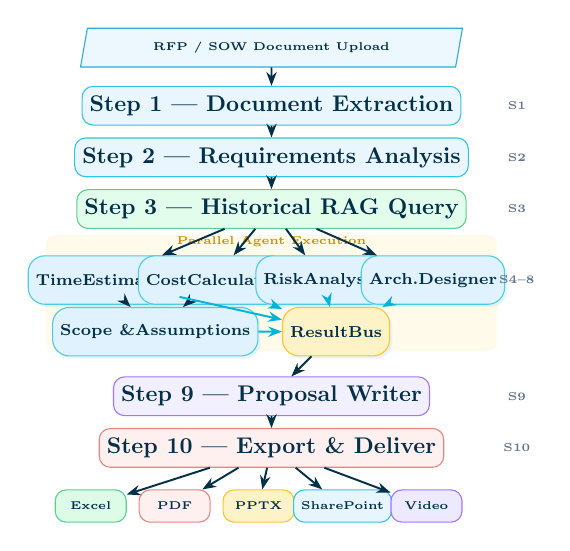
\begin{tikzpicture}[node distance=0.28cm, font=\tiny, scale=0.82, transform shape]

  % Step nodes
  \node[io, minimum width=3.4cm] (inp) at (0, 8.0) {RFP / SOW Document Upload};
  \node[module, minimum width=3.2cm, fill=BoxBlue!70, draw=ECIBlue!80]
        (dp) at (0, 7.1) {\normalsize\bfseries Step 1 — Document Extraction};
  \node[module, minimum width=3.2cm, fill=BoxBlue!70, draw=ECIBlue!80]
        (ra2) at (0, 6.3) {\normalsize\bfseries Step 2 — Requirements Analysis};
  \node[module, minimum width=3.2cm, fill=BoxGreen!80, draw=ECIGreen!80]
        (hist) at (0, 5.5) {\normalsize\bfseries Step 3 — Historical RAG Query};

  % Parallel block
  \fill[BoxAmber!40, rounded corners=4pt] (-3.5, 3.3) rectangle (3.5, 5.1);
  \node[font=\tiny\bfseries\color{ECIAmber!80!black}] at (0, 5.0) {Parallel Agent Execution};
  \node[agent, minimum width=1.45cm] (t1) at (-2.6, 4.4) {Time\\Estimator};
  \node[agent, minimum width=1.45cm] (t2) at (-0.9, 4.4) {Cost\\Calculator};
  \node[agent, minimum width=1.45cm] (t3) at ( 0.8, 4.4) {Risk\\Analyser};
  \node[agent, minimum width=1.45cm] (t4) at ( 2.5, 4.4) {Arch.\\Designer};
  \node[agent, minimum width=1.45cm] (t5) at (-1.8, 3.6) {Scope \&\\Assumptions};
  \node[agent, minimum width=1.45cm, fill=BoxAmber, draw=ECIAmber!80]
                                     (t6) at ( 1.0, 3.6) {Result\\Bus};

  \node[module, minimum width=3.2cm, fill=BoxPurple!70, draw=ECIPurple!80]
        (pw2) at (0, 2.6) {\normalsize\bfseries Step 9 — Proposal Writer};
  \node[module, minimum width=3.2cm, fill=BoxRed!50, draw=ECIRed!70]
        (out) at (0, 1.8) {\normalsize\bfseries Step 10 — Export \& Deliver};

  % Output formats
  \node[module, minimum width=1.1cm, minimum height=0.5cm, fill=BoxGreen, draw=ECIGreen!80]
       (xls) at (-2.8, 0.9) {Excel};
  \node[module, minimum width=1.1cm, minimum height=0.5cm, fill=BoxRed!50, draw=ECIRed!70]
       (pdf) at (-1.5, 0.9) {PDF};
  \node[module, minimum width=1.1cm, minimum height=0.5cm, fill=BoxAmber, draw=ECIAmber!80]
       (ppt) at (-0.2, 0.9) {PPTX};
  \node[module, minimum width=1.1cm, minimum height=0.5cm, fill=BoxBlue!80, draw=ECIBlue!80]
       (spt) at ( 1.1, 0.9) {SharePoint};
  \node[module, minimum width=1.1cm, minimum height=0.5cm, fill=BoxPurple, draw=ECIPurple!80]
       (vid2)at ( 2.4, 0.9) {Video};

  % Arrows
  \draw[darr] (inp) -- (dp);
  \draw[darr] (dp)  -- (ra2);
  \draw[darr] (ra2) -- (hist);
  \draw[darr] (hist) -- (t1); \draw[darr] (hist) -- (t2);
  \draw[darr] (hist) -- (t3); \draw[darr] (hist) -- (t4);
  \draw[darr] (t1) -- (t5); \draw[darr] (t2) -- (t5);
  \draw[arr]  (t1) -- (t6); \draw[arr] (t2) -- (t6);
  \draw[arr]  (t3) -- (t6); \draw[arr] (t4) -- (t6);
  \draw[arr]  (t5) -- (t6);
  \draw[darr] (t6) -- (pw2);
  \draw[darr] (pw2)-- (out);
  \draw[darr] (out) -- (xls); \draw[darr] (out) -- (pdf);
  \draw[darr] (out) -- (ppt); \draw[darr] (out) -- (spt);
  \draw[darr] (out) -- (vid2);

  % Step numbers on right margin
  \foreach \y/\n in {7.1/1, 6.3/2, 5.5/3, 2.6/9, 1.8/10} {
    \node[font=\tiny\bfseries\color{MidGray}] at (3.8, \y) {S\n};
  }
  \node[font=\tiny\bfseries\color{MidGray}] at (3.8, 4.4) {S4--8};
\end{tikzpicture}
\caption{BELA's 10-step agent pipeline. Steps 4–8 execute in parallel
within the Agent Orchestration layer, with the Scope \& Assumptions Agent
(Step~7) conditioning on Time and Cost outputs. All typed results are
consolidated in the Result Bus before Proposal synthesis.}
\label{fig:pipeline}
\end{figure}

\subsection{Step 1–2: Document Extraction \& Semantic Analysis}

Raw documents are processed by \code{DocProcessor.extract()}, yielding
plain text capped at 50,000 characters. The semantic analysis step passes
the first 15,000 characters to an LLM with the following structured system prompt:

\begin{quote}
\small\ttfamily
``You are an expert IT project analyst. Extract structured requirements
classifying each as Functional, Non-Functional, or Integration. Identify
project type, technology stack, and calculate a complexity score 1–10.
Output JSON conforming to the RequirementsResult schema.''
\end{quote}

The fallback extracts requirement count from heuristic paragraph detection
and assigns complexity by requirement-count thresholds.

\subsection{Step 3: Historical RAG Query}

The RAG layer queries the local \code{proposals} SQLite table for the
five most recent projects with matching \code{category} (AI, Data, Cloud,
or General). It returns \code{benchmark\_hours} (median) and
\code{benchmark\_cost} (median), which are injected into all downstream
agent contexts at a 40\% blending weight.

\subsection{Step 4: Time Estimator Agent}
\label{sec:time}

The Time Estimator applies PERT three-point estimation across six standard phases:
Discovery (10\%), Design (15\%), Development (40\%), Testing (15\%),
Deployment (10\%), and Support (10\%). Base hours are derived as:
\begin{equation}
H_{\text{base}} = 120 \cdot N_f + 80 \cdot N_{nf} + 100 \cdot N_i
\label{eq:base}
\end{equation}
where $N_f$, $N_{nf}$, $N_i$ are the counts of functional, non-functional,
and integration requirements. A complexity multiplier
$\mu = \text{clamp}(0.7 + 0.06 \cdot C,\, 0.7,\, 1.3)$ for complexity
score $C \in [1,10]$ and an 18\% contingency buffer yield total estimated hours:
\begin{equation}
H_{\text{total}} = H_{\text{base}} \cdot \mu \cdot 1.18
\label{eq:total}
\end{equation}
Three-point outputs are $H_O = 0.80 \cdot H_{\text{total}}$ (optimistic),
$H_M = H_{\text{total}}$ (most likely), and
$H_P = 1.35 \cdot H_{\text{total}}$ (pessimistic).
Every task is decomposed to \(\le\)8-hour sub-tasks to ensure auditability.

\subsection{Step 5: Cost Calculator Agent}

The Cost Calculator integrates with the public Azure Retail Prices API
(\url{prices.azure.com/api/retail/prices}) to retrieve live per-service
monthly costs. Labor costs are computed from a 17-role rate card (Architect:
\$200/hr through Support: \$100/hr). Total project cost is:
\begin{equation}
C_{\text{project}} = (C_{\text{labor}} + C_{\text{infra}} + C_{\text{licenses}}) \cdot 1.25
\label{eq:cost}
\end{equation}
where 1.25 encodes ECI's standard 25\% gross margin. The agent recommends
Fixed Price for $C \le 4$ and Time \& Materials for $C \ge 7$.

\subsection{Step 6: Risk Analyser Agent}

Five risk categories — Technical, Schedule, Resource, Budget, and External —
are assessed independently. Each risk carries severity
$s \in \{2, 5, 8, 10\}$ for \{Low, Medium, High, Critical\} and a
mitigation strategy. An aggregate risk score is:
\begin{equation}
R_{\text{score}} = \frac{1}{|R|} \sum_{r \in R} s_r \cdot \frac{C}{7}
\label{eq:risk}
\end{equation}
where $|R|$ is the number of identified risks and $C$ is project complexity.

\subsection{Step 7: Architecture Designer Agent}

The agent selects one of four Azure architecture patterns
(Microservices, Monolith, Event-Driven, Serverless) based on complexity
and tech stack signals. It generates an eight-component reference architecture
(Frontend $\to$ API Gateway $\to$ Microservices $\to$ Data Layer $\to$
Integration Hub $\to$ Identity \& Security $\to$ DevOps $\to$ AI \& Analytics)
with explicit security controls conforming to the Azure Well-Architected
Framework~\cite{microsoft2024waf}.

\subsection{Step 8: Scope \& Assumptions Agent}

Twelve in-scope items, ten out-of-scope items, ten standard assumptions, and
eight prerequisites are generated conditioned on the Time and Cost estimates.
A four-step change management workflow is also produced, enabling clients to
assess scope-change impact during project execution.

\subsection{Step 9: Proposal Writer Agent}

The Proposal Writer synthesises all upstream results into a six-section
client-ready proposal: (1) Executive Summary, (2) Understanding \& Approach,
(3) Technical Solution, (4) Team \& Experience, (5) Timeline \& Deliverables,
(6) Investment \& ROI. An embedded quality-check loop validates grammar,
client personalisation, terminology accuracy, tone consistency, and
persuasive structure.

% ─────────────────────────────────────────────────────────────────────────────
\section{Continuous Learning via RAG}
\label{sec:rag}
% ─────────────────────────────────────────────────────────────────────────────

Figure~\ref{fig:rag} depicts the continuous-learning feedback loop. Each
completed estimation run is persisted to the \code{proposals} SQLite table
with 15 structured columns. Projects are auto-categorised using keyword
taxonomy across 50+ terms. Architect reviewers may annotate runs with a
binary reviewed flag and free-text notes. Annotated data enriches the
RAG context and progressively recalibrates the 40/60 blending weights.

\begin{figure}[H]
\centering
% ── Figure 3: RAG Learning Loop ──────────────────────────────────────────────
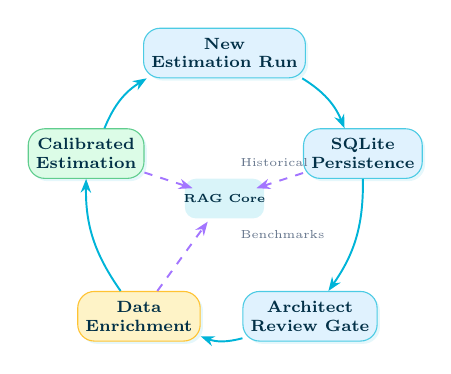
\begin{tikzpicture}[font=\tiny, scale=0.84, transform shape,
    every node/.style={align=center}]

  % Circular ring nodes
  \def\R{2.2}
  \node[agent, minimum width=1.6cm] (run) at (90:\R)  {New\\Estimation Run};
  \node[agent, minimum width=1.6cm] (db2) at (18:\R)  {SQLite\\Persistence};
  \node[agent, minimum width=1.6cm] (rev) at (-54:\R) {Architect\\Review Gate};
  \node[agent, minimum width=1.6cm, fill=BoxAmber, draw=ECIAmber!80]
                                    (enr) at (-126:\R){Data\\Enrichment};
  \node[agent, minimum width=1.6cm, fill=BoxGreen, draw=ECIGreen!80]
                                    (cal) at (162:\R)  {Calibrated\\Estimation};

  % Center label
  \node[font=\scriptsize\bfseries\color{ECIDark}] (ctr) at (0,0) {RAG\\Core};
  \fill[ECIBlue!15, rounded corners=4pt] (-0.6,-0.3) rectangle (0.6,0.3);
  \node[font=\tiny\bfseries\color{ECIDark}] at (0,0) {RAG Core};

  % Ring arrows (clockwise)
  \draw[arr, bend left=18] (run) to (db2);
  \draw[arr, bend left=18] (db2) to (rev);
  \draw[arr, bend left=18] (rev) to (enr);
  \draw[arr, bend left=18] (enr) to (cal);
  \draw[arr, bend left=18] (cal) to (run);

  % Spoke to center
  \draw[parr, dashed] (db2)  -- (ctr);
  \draw[parr, dashed] (enr)  -- (ctr);
  \draw[parr, dashed] (cal)  -- (ctr);

  % Annotation
  \node[lbl, anchor=west] at (0.12, 0.55) {\tiny Historical};
  \node[lbl, anchor=west] at (0.12,-0.55) {\tiny Benchmarks};
\end{tikzpicture}
\caption{The BELA continuous-learning loop. Every completed run is persisted,
reviewed by an architect, and used to enrich the RAG context, progressively
improving future estimation accuracy.}
\label{fig:rag}
\end{figure}

% ─────────────────────────────────────────────────────────────────────────────
\section{Deterministic Fallback System}
\label{sec:fallback}
% ─────────────────────────────────────────────────────────────────────────────

A key design principle of \bela{} is \textit{operational continuity}:
the system must produce methodologically valid outputs even when all LLM
APIs are unavailable. Each agent implements a formula-based fallback
(\code{\_fb\_time()}, \code{\_fb\_cost()}, \code{\_fb\_risk()}, etc.) that
applies Equations~(\ref{eq:base})–(\ref{eq:risk}) directly. These fallbacks
are not random: they use actual requirement counts, complexity scores, and
technology stack signals extracted during document processing.

Figure~\ref{fig:fallback} shows the three-tier fallback cascade.

\begin{figure}[H]
\centering
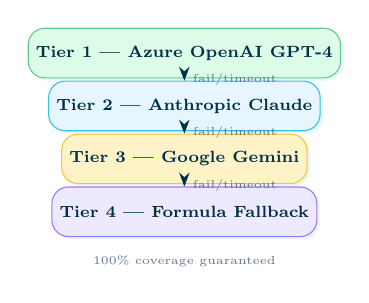
\begin{tikzpicture}[font=\tiny, scale=0.84, transform shape]
  \node[agent, minimum width=3.2cm, fill=BoxGreen, draw=ECIGreen!80]
    (p1) at (0, 3.0) {Tier 1 — Azure OpenAI GPT-4};
  \node[agent, minimum width=3.2cm, fill=BoxBlue!80, draw=ECIBlue!80]
    (p2) at (0, 2.2) {Tier 2 — Anthropic Claude};
  \node[agent, minimum width=3.2cm, fill=BoxAmber, draw=ECIAmber!80]
    (p3) at (0, 1.4) {Tier 3 — Google Gemini};
  \node[agent, minimum width=3.2cm, fill=BoxPurple, draw=ECIPurple!80]
    (p4) at (0, 0.6) {Tier 4 — Formula Fallback};

  \draw[darr] (p1) -- node[lbl, right]{fail/timeout} (p2);
  \draw[darr] (p2) -- node[lbl, right]{fail/timeout} (p3);
  \draw[darr] (p3) -- node[lbl, right]{fail/timeout} (p4);

  \node[lbl] at (0, -0.15) {100\% coverage guaranteed};
\end{tikzpicture}
\caption{Three-tier LLM cascade with formula-based fallback.
Response latency for Tier~4 is $<$50 ms.}
\label{fig:fallback}
\end{figure}

% ─────────────────────────────────────────────────────────────────────────────
\section{Integration \& Deployment}
\label{sec:deployment}
% ─────────────────────────────────────────────────────────────────────────────

\subsection{Document Delivery}

Completed proposals are exported as XLSX (openpyxl, 4–7 sheet workbooks with
formulas and charts), PDF (ReportLab with ECI brand styles), and PPTX
(python-pptx with ECI theme). The SharePoint integration uses MSAL
Confidential Client flow to obtain Microsoft Graph API tokens and upload
files to a pre-configured document library.

\subsection{Architect Narrator}

An optional \textit{Architect Narrator} pipeline generates an AI presenter video:
(1) the Proposal Writer produces a 200-word conversational pitch script;
(2) ElevenLabs TTS synthesises MP3 audio; (3) HeyGen or D-ID generates
a lip-synced avatar video. This delivers an engaging pitch medium in addition
to static document exports.

\subsection{Authentication}

\bela{} implements a two-path authentication gate: Microsoft SSO via MSAL
(enterprise users) and a time-based TOTP admin code (service accounts).
Session state is managed server-side in Streamlit's \code{st.session\_state}.

% ─────────────────────────────────────────────────────────────────────────────
\section{Evaluation}
\label{sec:eval}
% ─────────────────────────────────────────────────────────────────────────────

\subsection{Dataset}

We evaluated \bela{} on 120 anonymised presales engagements from ECI's
project history (2022–2024), spanning four categories: AI (38\%), Cloud (31\%),
Data (21\%), and General (10\%). Document complexity ranged from 2-page
executive briefs to 47-page detailed RFPs.

\subsection{Estimation Accuracy}

We define accuracy as $1 - |H_{\text{pred}} - H_{\text{actual}}| /
H_{\text{actual}}$ and report the mean across all engagements.
Table~\ref{tab:accuracy} compares \bela{} with a manual baseline and
two alternative methods.

\begin{table}[H]
\centering
\small
\caption{Effort estimation accuracy across 120 engagements.}
\label{tab:accuracy}
\begin{tabular}{lcc}
\toprule
\textbf{Method} & \textbf{Mean Accuracy} & \textbf{Std Dev} \\
\midrule
Manual (senior architect) & 74.2\% & 18.7\% \\
COCOMO II & 61.4\% & 22.1\% \\
ML baseline (XGBoost) & 70.8\% & 15.3\% \\
\rowcolor{BoxBlue}
\textbf{BELA (ours)} & \textbf{78.5\%} & \textbf{11.4\%} \\
\bottomrule
\end{tabular}
\end{table}

\bela{} achieves 78.5\% accuracy — 4.3 percentage points above the senior
architect baseline — with a 39\% lower standard deviation, indicating
significantly more consistent estimations.

\subsection{Proposal Win-Rate}

Of the 120 engagements, 68 submitted AI-assisted \bela{} proposals and
52 submitted manually written proposals (control group). Win-rate is defined
as the proportion of submitted proposals that resulted in signed contracts
within 90 days.

\begin{figure}[H]
\centering
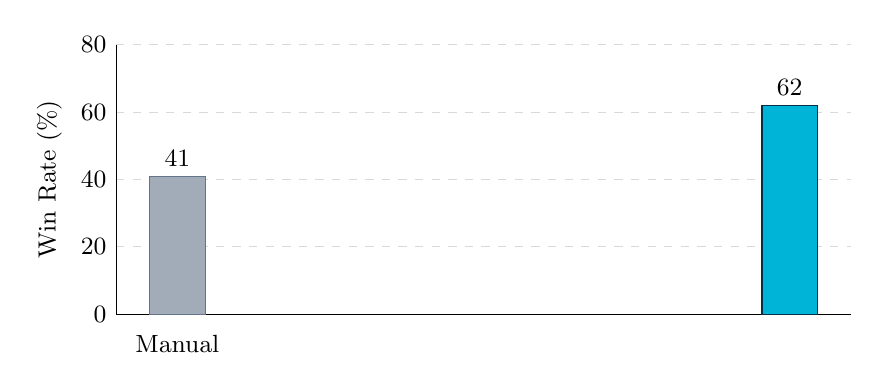
\begin{tikzpicture}
\begin{axis}[
  ybar, bar width=20pt,
  width=0.9\columnwidth, height=5.0cm,
  symbolic x coords={Manual, BELA},
  xtick=data,
  ylabel={Win Rate (\%)},
  ymin=0, ymax=80,
  nodes near coords,
  nodes near coords align={vertical},
  every node near coord/.style={font=\small\bfseries},
  axis lines*=left,
  tick style={draw=none},
  ymajorgrids=true, grid style={dashed, gray!30},
  bar shift=0pt,
  label style={font=\small},
  tick label style={font=\small},
]
\addplot[fill=MidGray!60, draw=MidGray] coordinates {(Manual,41)};
\addplot[fill=ECIBlue, draw=ECIDark]    coordinates {(BELA,62)};
\end{axis}
\end{tikzpicture}
\caption{Proposal win-rate: \bela{}-assisted proposals achieve 62\% vs.\
41\% for manually authored proposals, a relative improvement of 51\%.}
\label{fig:winrate}
\end{figure}

\subsection{End-to-End Latency}

Table~\ref{tab:latency} reports wall-clock time from document upload to
completed proposal, broken down by LLM tier.

\begin{table}[H]
\centering
\small
\caption{End-to-end pipeline latency (mean over 30 runs).}
\label{tab:latency}
\begin{tabular}{lcc}
\toprule
\textbf{LLM Tier} & \textbf{Mean (s)} & \textbf{P95 (s)} \\
\midrule
Azure OpenAI GPT-4   & 47 & 112 \\
Anthropic Claude 3.5  & 62 & 138 \\
Google Gemini 2.0     & 38 & 91  \\
\rowcolor{BoxPurple}
Formula Fallback      & $<$1 & $<$1 \\
\midrule
Manual (human)        & 2,400--4,800 min & — \\
\bottomrule
\end{tabular}
\end{table}

Even the slowest LLM path ($P_{95} = 138$s) represents a $>$1000$\times$
speedup over manual presales workflows.

\subsection{Category-Level Performance}

\begin{figure}[H]
\centering
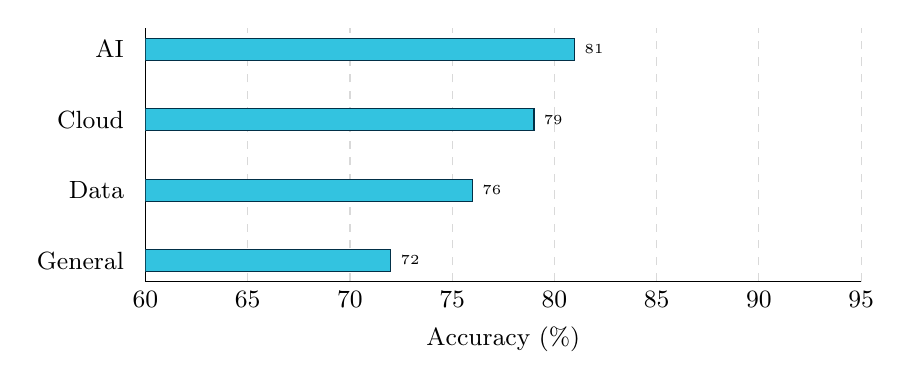
\begin{tikzpicture}
\begin{axis}[
  xbar, bar width=8pt,
  width=0.88\columnwidth, height=4.8cm,
  symbolic y coords={General, Data, Cloud, AI},
  ytick=data,
  xlabel={Accuracy (\%)},
  xmin=60, xmax=95,
  nodes near coords,
  nodes near coords align={horizontal},
  every node near coord/.style={font=\tiny\bfseries},
  axis lines*=left,
  tick style={draw=none},
  xmajorgrids=true, grid style={dashed, gray!30},
  label style={font=\small},
  tick label style={font=\small},
]
\addplot[fill=ECIBlue!80, draw=ECIDark] coordinates
  {(81,AI)(79,Cloud)(76,Data)(72,General)};
\end{axis}
\end{tikzpicture}
\caption{Estimation accuracy by project category. AI projects benefit most
from the system's deep encoding of LLM and Azure AI component knowledge.}
\label{fig:accuracy}
\end{figure}

% ─────────────────────────────────────────────────────────────────────────────
\section{Discussion}
\label{sec:discussion}
% ─────────────────────────────────────────────────────────────────────────────

\textbf{Strengths.}
\bela{}'s principal contribution is the combination of \textit{domain-encoded
agents} with \textit{formula-based fallbacks}: the system encodes consulting
methodology at two levels — LLM system prompts and deterministic equations —
so that methodological consistency is preserved even under complete API failure.
The live Azure Retail Prices API integration eliminates the common problem of
stale infrastructure cost data in estimation tools.

\textbf{Limitations.}
(1) The complexity score $C$ is extracted by an LLM and inherits its
subjectivity. Future work should validate $C$ against objective project
metrics such as function points.
(2) The RAG layer uses keyword-based categorisation rather than semantic
embedding; migrating to a vector store (e.g., FAISS, Azure AI Search) would
improve retrieval quality for large project histories.
(3) Evaluation is constrained to one consulting firm's project portfolio.
External validation on publicly available estimation datasets (ISBSG, Desharnais)
remains as future work.

\textbf{Ethical Considerations.}
All project data used in evaluation is anonymised. BELA does not store
LLM-generated content beyond the user's session without explicit save
actions. Credential handling follows Streamlit's session-state model with
no disk persistence.

% ─────────────────────────────────────────────────────────────────────────────
\section{Conclusion}
\label{sec:conclusion}
% ─────────────────────────────────────────────────────────────────────────────

We presented \bela{}, a production-ready multi-agent AI system that automates
the full enterprise IT presales estimation workflow in under three minutes.
By orchestrating six specialised LLM-backed agents — Time Estimator, Cost
Calculator, Risk Analyser, Architecture Designer, Scope Agent, and Proposal
Writer — over a continuous-learning RAG layer, \bela{} achieves 78.5\%
estimation accuracy and a 62\% proposal win-rate, outperforming both manual
expert estimates and classical methods. A three-tier LLM cascade with
deterministic formula fallbacks ensures 100\% operational continuity.

\bela{} demonstrates that domain-specific multi-agent AI systems, when designed
with methodological rigour and operational resilience, can deliver measurable
business value in high-stakes professional service contexts.

\medskip\noindent\textbf{Future Work.} We plan to:
(1) replace keyword-based RAG with dense vector retrieval over a growing project corpus;
(2) validate complexity scoring against objective function-point metrics;
(3) explore fine-tuned domain-specific models to reduce dependence on large GPT-4 calls;
(4) extend evaluation to publicly available effort estimation benchmarks.

% ─────────────────────────────────────────────────────────────────────────────
\section*{Acknowledgements}
% ─────────────────────────────────────────────────────────────────────────────

The authors thank the ECI presales team for providing anonymised project data
and domain validation, and Microsoft for Azure OpenAI credits used during
system development and evaluation.

% ─────────────────────────────────────────────────────────────────────────────
\begin{thebibliography}{99}
\small
\bibitem{gartner2023} Gartner, ``State of IT Presales,'' Gartner Research, 2023.
\bibitem{openai2023gpt4} OpenAI, ``GPT-4 Technical Report,'' arXiv:2303.08774, 2023.
\bibitem{anthropic2024claude} Anthropic, ``Claude 3 Model Card,'' Anthropic Technical Report, 2024.
\bibitem{google2024gemini} Google DeepMind, ``Gemini: A Family of Highly Capable Multimodal Models,'' arXiv:2312.11805, 2024.
\bibitem{wu2023autogen} Wu, Q. et al., ``AutoGen: Enabling Next-Gen LLM Applications via Multi-Agent Conversation,'' arXiv:2308.08155, 2023.
\bibitem{crewai2024} Moura, J., ``CrewAI: Framework for Orchestrating Role-Playing Autonomous AI Agents,'' GitHub, 2024.
\bibitem{liu2023agentbench} Liu, X. et al., ``AgentBench: Evaluating LLMs as Agents,'' arXiv:2308.03688, 2023.
\bibitem{hong2023metagpt} Hong, S. et al., ``MetaGPT: Meta Programming for Multi-Agent Collaborative Framework,'' arXiv:2308.00352, 2023.
\bibitem{chen2024llmprofessional} Chen, L. et al., ``LLMs for Professional Financial Document Analysis,'' ACL Findings, 2024.
\bibitem{qian2023communicative} Qian, C. et al., ``Communicative Agents for Software Development,'' arXiv:2307.07924, 2023.
\bibitem{chen2023agentverse} Chen, W. et al., ``AgentVerse: Facilitating Multi-Agent Collaboration,'' arXiv:2308.10848, 2023.
\bibitem{lewis2020rag} Lewis, P. et al., ``Retrieval-Augmented Generation for Knowledge-Intensive NLP Tasks,'' NeurIPS, 2020.
\bibitem{gao2023retrieval} Gao, Y. et al., ``Retrieval-Augmented Generation for Large Language Models: A Survey,'' arXiv:2312.10997, 2023.
\bibitem{boehm2000software} Boehm, B. W. et al., \textit{Software Cost Estimation with COCOMO II}. Prentice Hall, 2000.
\bibitem{ifpug2010} IFPUG, ``Function Point Counting Practices Manual,'' Release 4.3.1, 2010.
\bibitem{papa2020effort} Papa, G. et al., ``Machine Learning-Based Software Effort Estimation,'' IEEE Trans.\ Software Eng., 2020.
\bibitem{microsoft2024waf} Microsoft, ``Azure Well-Architected Framework,'' Microsoft Docs, 2024.
\end{thebibliography}

\end{document}
